\documentclass{sig-alternate-sigmod09}

\usepackage[bookmarks=true,pdfborder= 0 0 0]{hyperref}

\usepackage{tikz}
\usetikzlibrary{calc,trees,positioning,arrows,chains,shapes.geometric,%
  decorations.pathreplacing,decorations.pathmorphing,shapes,%
  matrix,shapes.symbols,plotmarks,decorations.markings,shadows}

\DeclareMathOperator{\atantwo}{atan2}

\hypersetup{
pdfauthor={Patrick Brosi},
pdfkeywords=,
pdftitle={An Approximation Algorithm for Metro Map Drawing},
pdfsubject={},
pdfcreator={},
pdfproducer={}
}

\begin{document}
\title{An Approximation Algorithm for Metro Map Drawing}

\numberofauthors{1}
%\author{Patrick Brosi\\\affaddr{University of Freiburg}\\\affaddr{Chair of Algorithms and Data Structures}}

\maketitle

\section{Abstract}

We investigate a novel approximative approach to the NP-hard problem of octilinear Metro Map drawing. Contrary to previous work, which usually relied on either local or global optimization techniques, we state the task as a (greedy) iterative shortest-path problem on a specially crafted octilinear grid graph, whose edge weights are locally updated after each iteration. While our results are not perfect, they come surprisingly close to previous work which used Integer Linear Programming to find a globally optimal solution, and do so fast. We state the basic idea of our approach, give some heuristics to improve the final result and evaluate our method on 10 cities around the world. As far as we are aware, our approach is the first non-global approach which guarantees octilinear results, albeit at the cost of not always finding a solution. The resulting schematic maps are rendered using previous work by us and are publicly accessible at http://bla.blubb.

\section{Introduction}

Lorem ipsum
\begin{figure}[t]
  \centering
	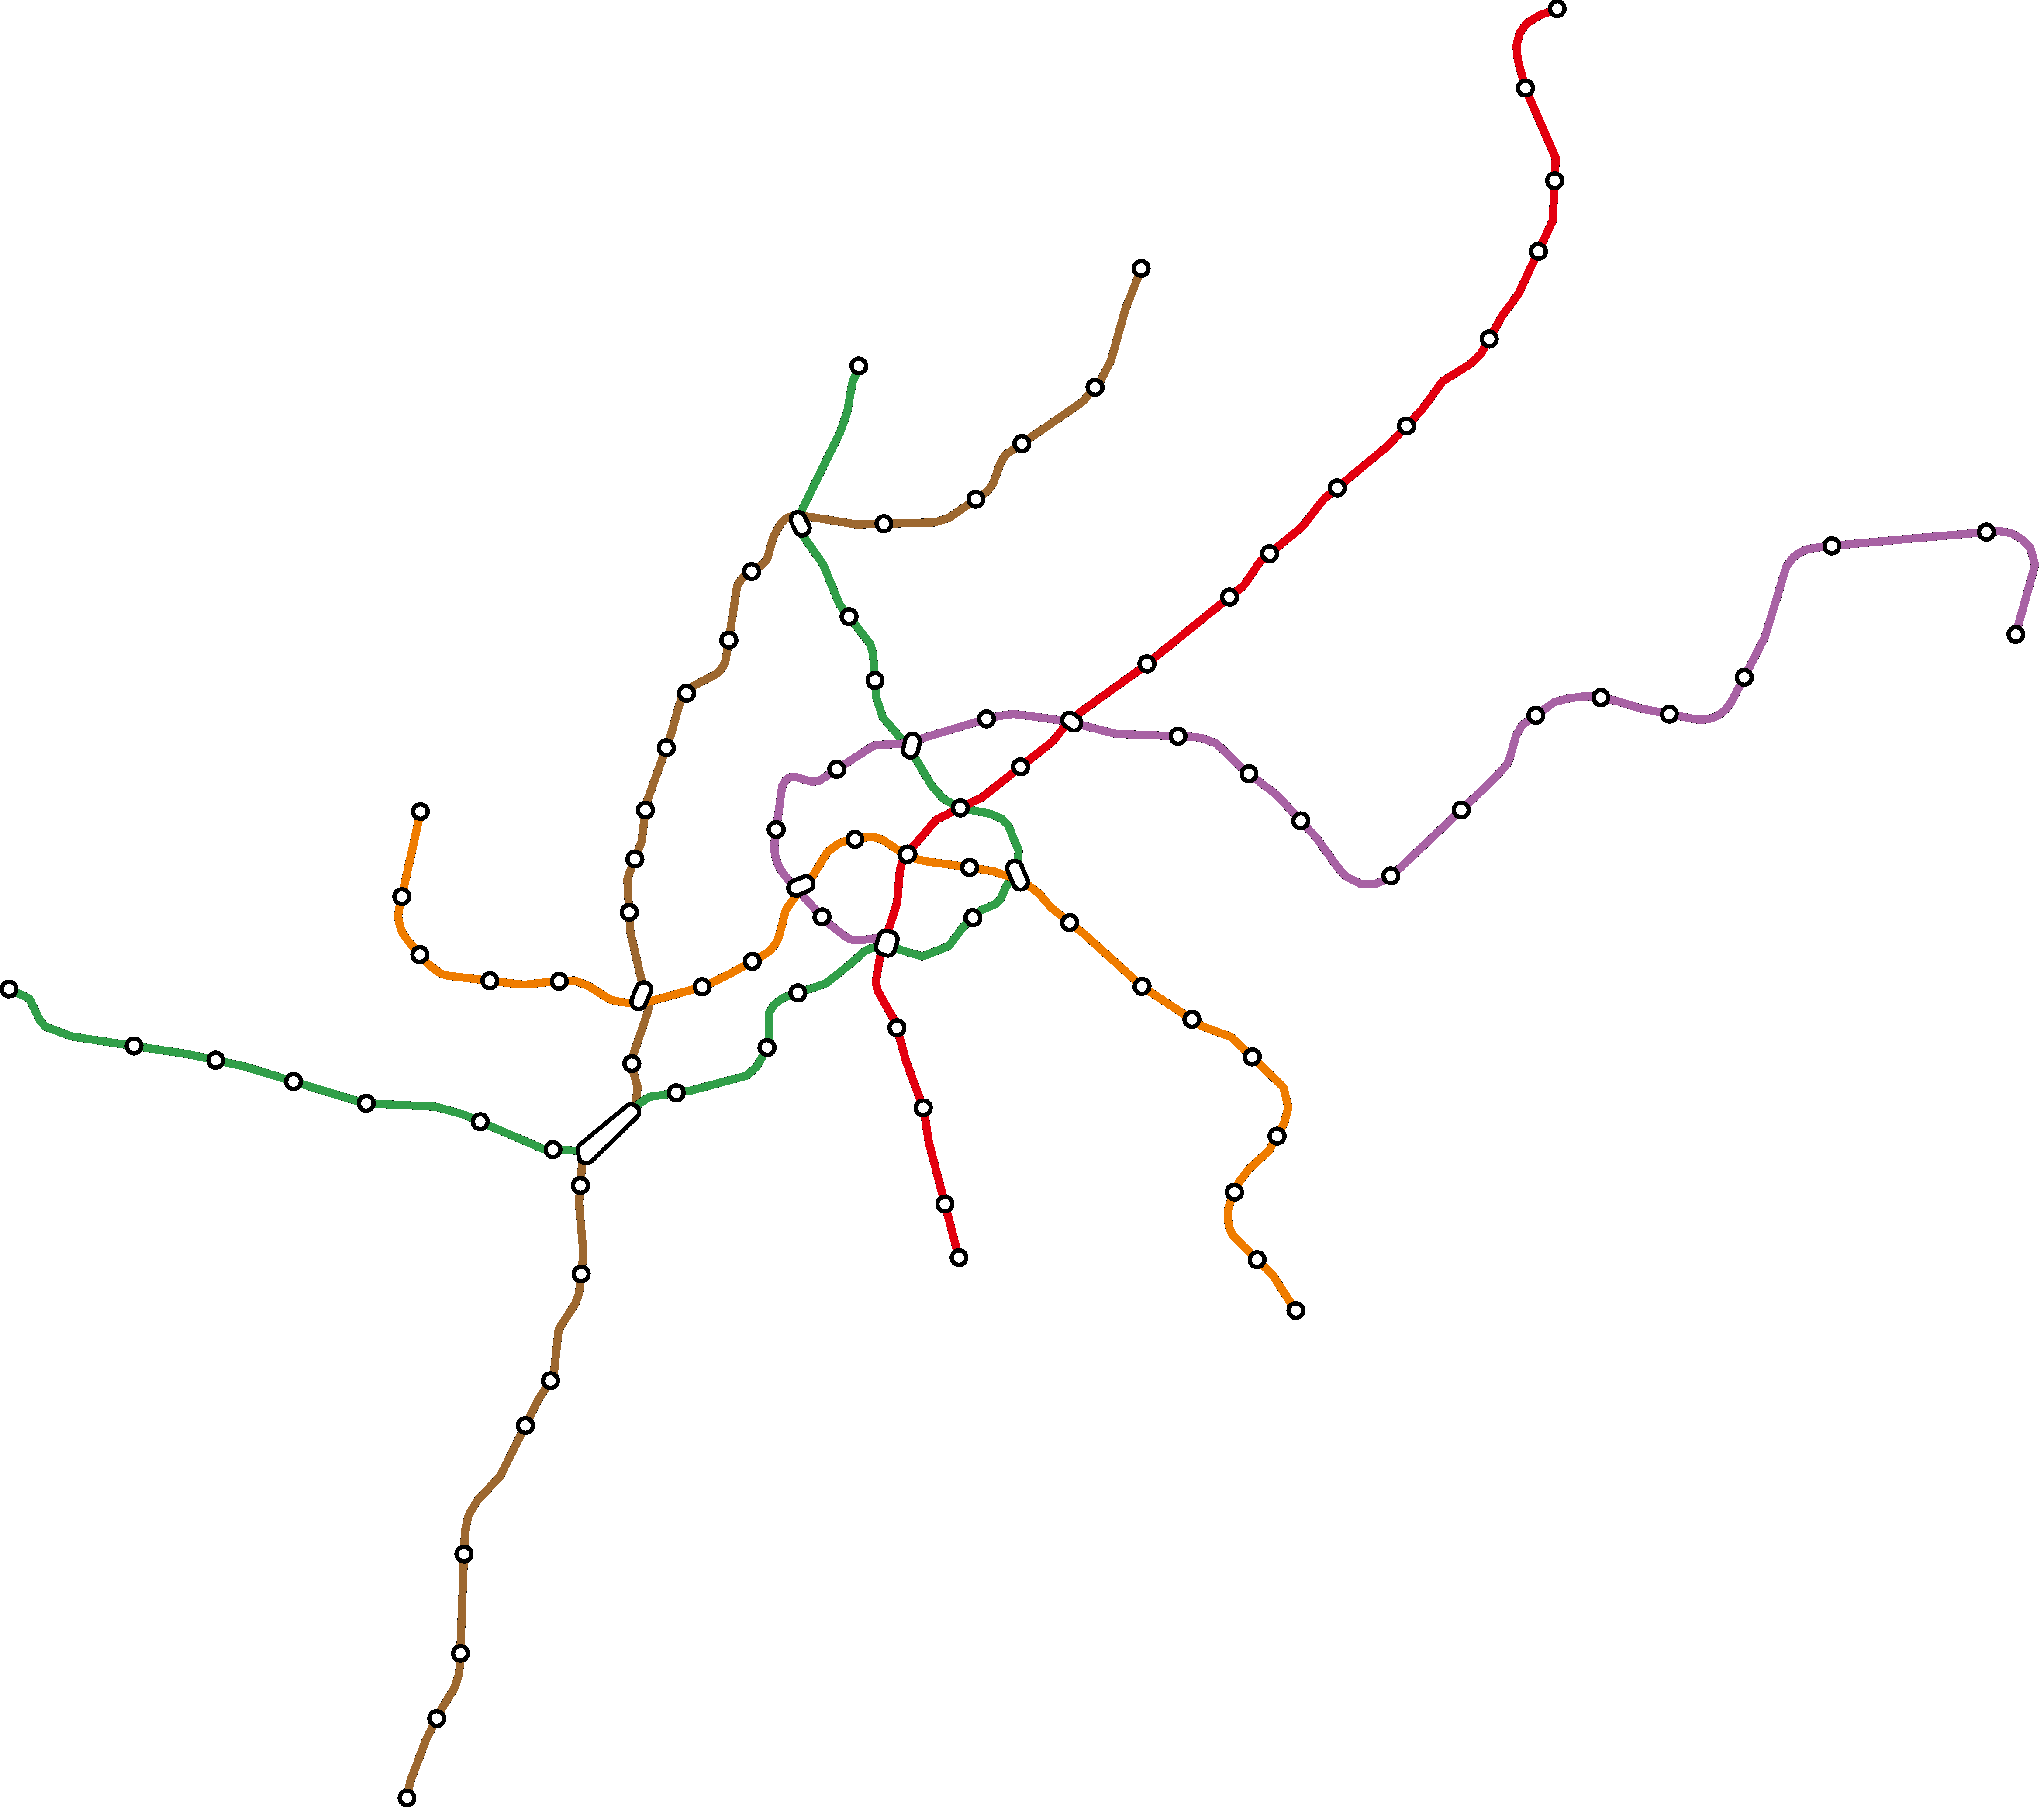
\includegraphics[width=0.474\textwidth]{figures/octi_input.pdf}
	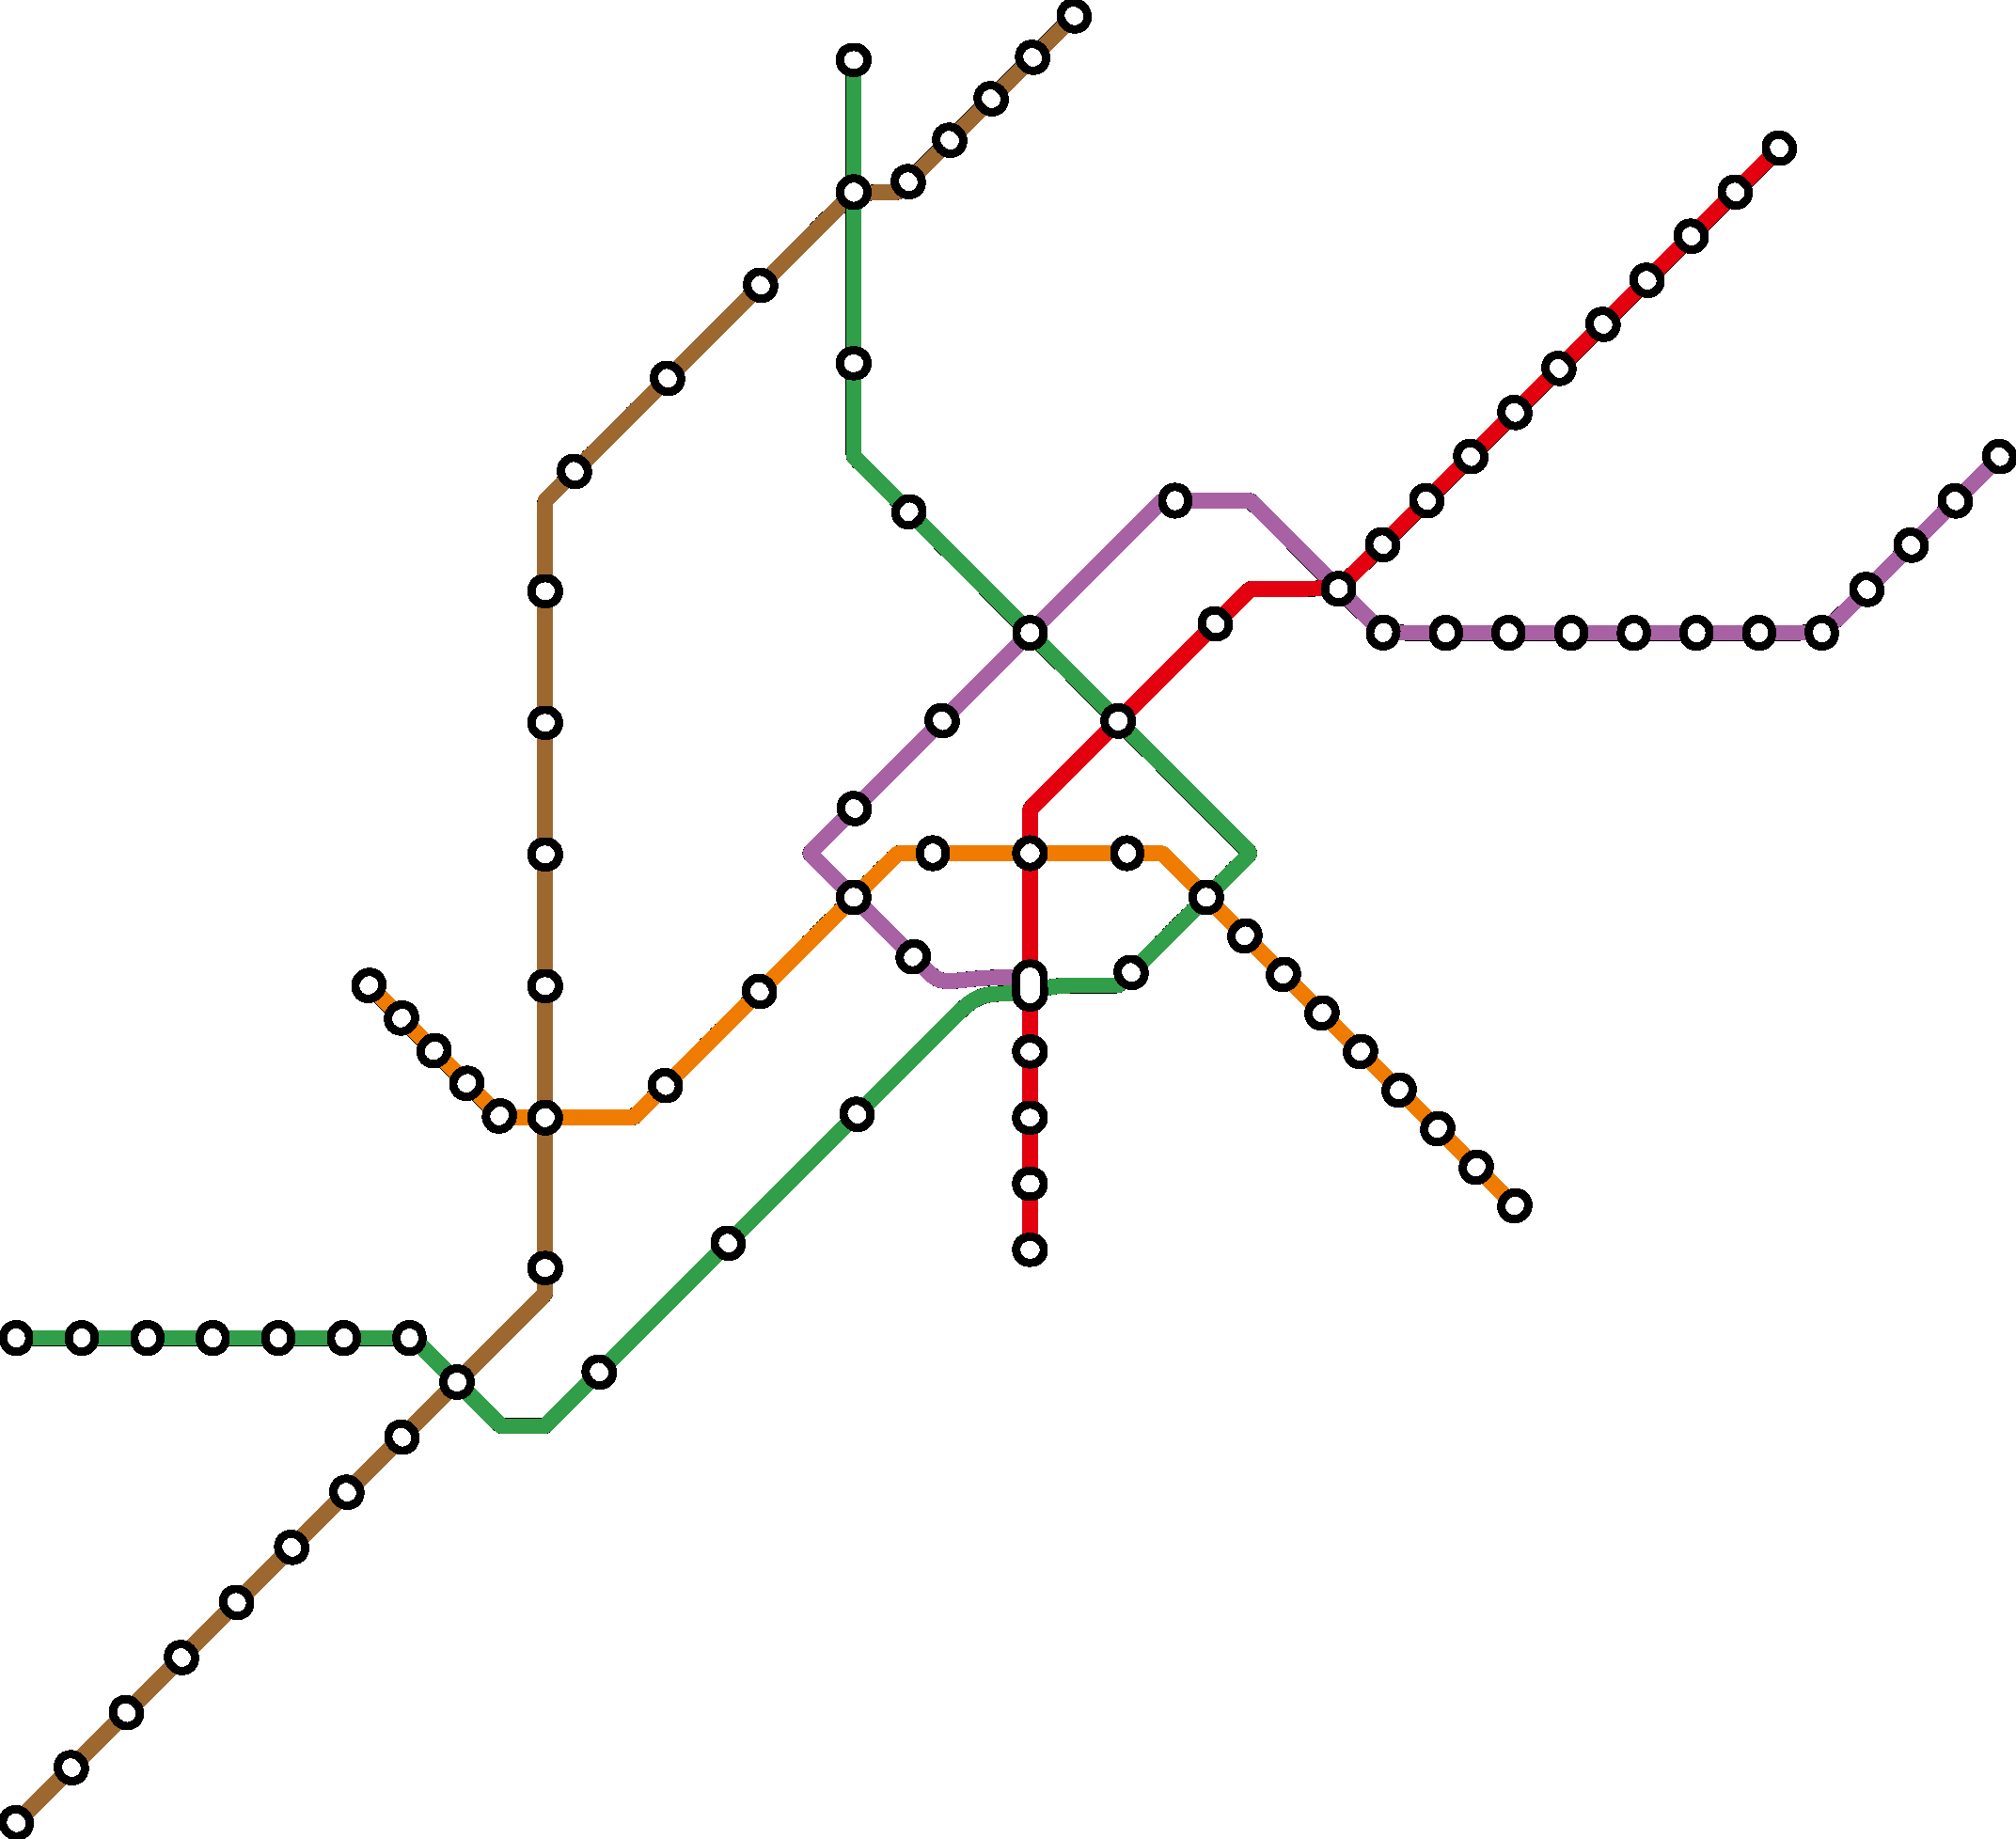
\includegraphics[width=0.474\textwidth]{figures/octi.pdf}
	\caption{The subway network of Vienna, rendered with our approach from raw timetable (GTFS) data (including stop positions).}
	\label{FIG:examplewien}
\end{figure}

\section{Problem definition}

Given an undirected planar graph $G = \{V, E\}$. We say $\mathcal{D}_G = \{p, c\}$ is a drawing of $G$, where $p(v) \in \mathbb{R}^2$ assigns a position to every node $v \in V$ and $c(e) = (q_0, q_1, ..., q_n)$, $q_i \in \mathbb{R}^2$ assigns a piecewise linear curve to every edge $e \in E$. The initial input drawing $\mathcal{D}_G$ assigns each node a real-world position, and each edge an (optional) real-world trajectory on a two-dimensional map plane. Our goal is to find a schematic drawing $\mathcal{D}'_G$ that resembles a classic Metro Map. This is usually formalized as a set of hard and soft constraints \cite{nb, ...}. The hard constraints may be summarized as:
\begin{enumerate}
\setlength\itemsep{.1em}
\item \emph{Octilinearity}. Each edge curve $c(e)$ may only consist of segments whose orientation is a multiple of $45^{\circ}$.
\item \emph{Topology preservation}. The input embedding should be respected. In particular, no crossings between edges should be introduced and non-incident edges should never share common points. This is often modelled as a minimum distance $d_{e}$ between non-incident edge curves and a minimum distance $d_{v}$ between node positions.
\end{enumerate}
Additionally, the following soft constraints are usually employed:
\begin{enumerate}
\setlength\itemsep{.1em}
\item \emph{Edge monotony}. Minimize the number of turns an edge has to take. Prefer large angles.
\item \emph{Geographical accuracy}. The original node positions should be distorted as little as possible.
\item \emph{} Balance the angular distribution of incident edges in nodes.
\item \emph{Map density}.
\end{enumerate}

This list of soft constraints does not claim to be complete. % some more info on additional constraints


\section{Related Work}

Survey Nöllenburg %http://i11www.iti.kit.edu/extra/publications/n-asamm-14.pdf
Survey Wolff %http://www1.pub.informatik.uni-wuerzburg.de/pub/wolff/pub/w-dsms-07.pdf
Hong et al., force-based approach
Stott's PhD
steiner trees! %https://www.researchgate.net/profile/Matthias_Mueller-Hannemann/publication/225160153_Approximation_of_Octilinear_Steiner_Trees_Constrained_by_Hard_and_Soft_Obstacles/links/0912f50cf248ec1193000000/Approximation-of-Octilinear-Steiner-Trees-Constrained-by-Hard-and-Soft-Obstacles.pdf

\section{Map Generation}

To find an octilinear drawing for some graph $G$, our algorithm proceeds in three basic steps: 1. Build a so-called octilinear grid graph $\Omega$ on which the drawing of a shortest path between two nodes is guaranteed to be octilinear and as smooth as possible. 2.) For an unsettled edge $e = \{u, v\}$ in $G$ find suitable nodes $u'$ and $v'$ in $\Omega$ and search for the shortest path from $u'$ to $v'$. 3. Based on the path found for $e$ in step 2, balance $\Omega$ locally. Mark $e$ as settled and greedily continue with step 2.

This section gives detailed descriptions of all steps involved. Section~\ref{SEC:} describes additional balancing constraints to preserve the original embedding and discusses heuristics to prevent dead-locks.

\subsection{Octilinear Grid Graph}

We start by constructing an auxiliary undirected graph $\Omega = \{V_\omega, E_\omega\}$ with a drawing $\mathcal{D}_\Omega = \{p_\omega, c_\omega\}$ in such a way that every possible path $(v_0, v_1, ..., v_n), v_i \in V_\Omega$ is automatically represented as an octilinear curve by concatenating $p_\omega(v_0)$, $p_\omega(v_0)$,$...$,$p_\omega(v_n)$. The graph in Fig.~\ref{FIG:gridgraph} trivially satisfies this: we simply define a $n\times m$ grid, add nodes $v_{n,m}$ to $V_\omega$ for every grid point and set $p_\omega(v_{n,m}) = (n, m)$. Each node $v_{n,m}$ is connected with its 8 direct neighbors (except at the grid boundaries) $N^0(v_{n,m}) ... N^7(v_{n, m})$, where $N^0(v_{n,m})$ is the ``north'' neighbor of $v_{n, m}$,  $N^1(v_{n,m})$ the ``north-east'' neighbor and so on, in clockwise fashion.

For each node, we set $p_\omega(v_{n, m}) = (n, m)$. The drawing for some edge $e = \{v_{n, m}, N^i(v_{n, m})\}$ is just a straight line connecting the adjacent nodes. We call the nodes $v_{n, m}$ grid nodes, and the edges connecting them grid edges.

To optimize soft constraint (1), we additionally want the total cost for a path from a node $v \in V_\omega$ to a node $u \in V_\omega$ to also reflect the total number of necessary turns. The penalty for a turn should be weighted by its degree - either $135^{\circ}$, $90^{\circ}$ or $45^{\circ}$. We call these penalties $p_{135}$, $p_{90}$ and $p_{45}$. A straight pass through a node should go unpunished, that is, $p_{180} = 0$. Since we aim for a ``smooth'' path through $G$ and want to favor obtuse angles, we require $p_{180} < p_{135} < p_{90} < p_{45}$. The smoothest octilinear path from $u$ to $v$ in $\Omega$ would then be just the shortest path between them.

\begin{figure}
  \centering
	$\vcenter{\hbox{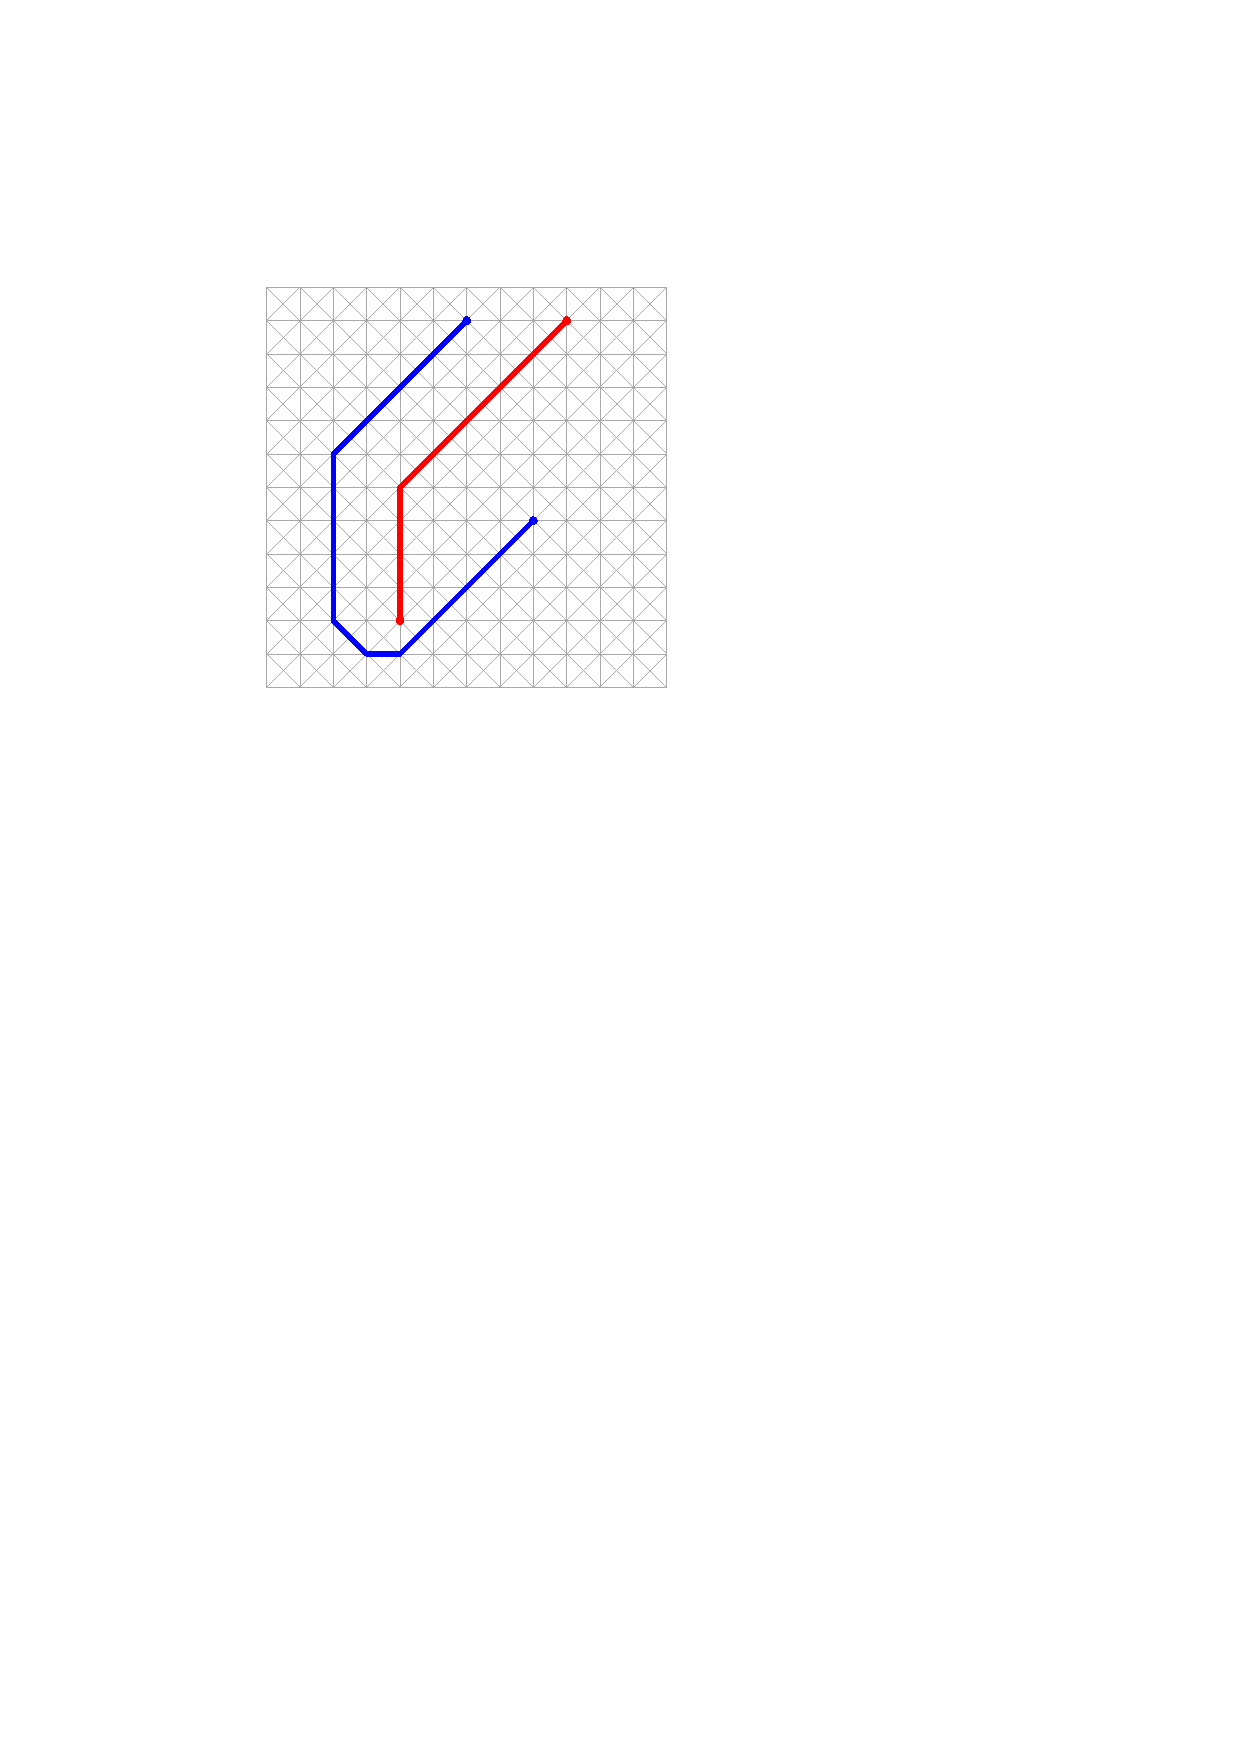
\includegraphics[width=0.474\textwidth]{figures/grid.pdf}}}$
	\caption{Left: A shortest path between $t$ and $u$ on a grid graph with uniform edge cost. Path turns are not minimized. Right: Two shortest path between $(t, u)$, and $(v, w)$ on our octilinear grid graph with uniform grid edge cost $1$ and additional path turn penalties $p_{135} = 1$, $p_{90} = 3$ and $p_{45} = 9$. Path $(t, u)$ acts as an obstacle for $(v, w)$.}
	\label{FIG:grids}
\end{figure}

We model this by adding 8 auxiliary port nodes $v_{n,m}^{0} ... v_{n,m}^{7}$ to every grid node $v_{n,m}$. Each port again corresponds to an outgoing angle in clockwise fashion and is connected to $v_{n, m}$ with a direct ``threshold'' edge $e_{n,m}^0 ... e_{n,m}^7$. We make sure that the cost for each of these threshold edges is bigger than the maximum cost of any other edge. This ensures that these edges are only used if we actually want to arrive in $v_{n,m}$. For paths passing through $v_{n,m}$, we connect each port $v_{n,m}^i$ with its 5 sibling ports at $90^{\circ}$ $135^{\circ}$, $180^{\circ}$, $225^{\circ}$ and $270^{\circ}$. We classify these edges by the angle of the turn they allow in $v_{n, m}$ - either $90^{\circ}$, $135^{\circ}$ or $180^{\circ}$. It will became apparent later on why we skip edges to allow a $45^{\circ}$ turn here.

A $180^{\circ}$ pass through $v_{n,m}$ coming from $N^k(v_{n, m})$ can now take the port edge $\epsilon^{180}(v_{n, m}^k)$ from $v_{n, m}^k$ to its $180^{\circ}$ sibling $v_{n, m}^{(k + 4) \mod 8}$ (Fig.~\ref{FIG:paths}, 1). Equally, a $90^{\circ}$ degree turn in $v_{n, m}$, coming from $v_{n, m}^k$ can take the port edge to $v_{n, m}^{(k + 2) \mod 8}$ (Fig.~\ref{FIG:paths}, 2) and so on.

As both a $45^{\circ}$ port edge and a $90^{\circ}$ port edge may be substituted by two (or more) cheaper edges, special care has to be applied to the modelling of the actual edge costs. For example, a $45^{\circ}$ turn can be simulated by first passing $v_{n, m}$ on a $180^{\circ}$ port edge, and then again on a $135^{\circ}$ port edge (Fig.~\ref{FIG:paths}, 3). As $p_{180} < p_{135} < p_{45}$, this path will be cheaper than $p_{45}$, undermining our penalty system. Similarily, a $90^{\circ}$ degree turn can be simulated by two cheaper $135^{\circ}$ port edges (Fig.~\ref{FIG:paths}, 4).

We call the actual edge costs for the 4 classes of port edges $c_0$, $c_{135}$, $c_{90}$ and $c_{45}$. To prevent the shortcuts described above, we make use of the fact that the absolute costs of these edges are irrelevant. Since they are modeled the same in every grid node and a path passing through (not going to) some $v_{n,m}$ has to take \emph{one} of them, we just have to make sure that the relative costs reflect the penalties we want to apply to the different turn angles, that is, $c_{135} - c_{180} = p_{135}$, $c_{90} - c_{180} = p_{90} = p_{135} + (c_{90}-c_{135})$ etc.

\begin{figure}[h]
  \centering
	$\vcenter{\hbox{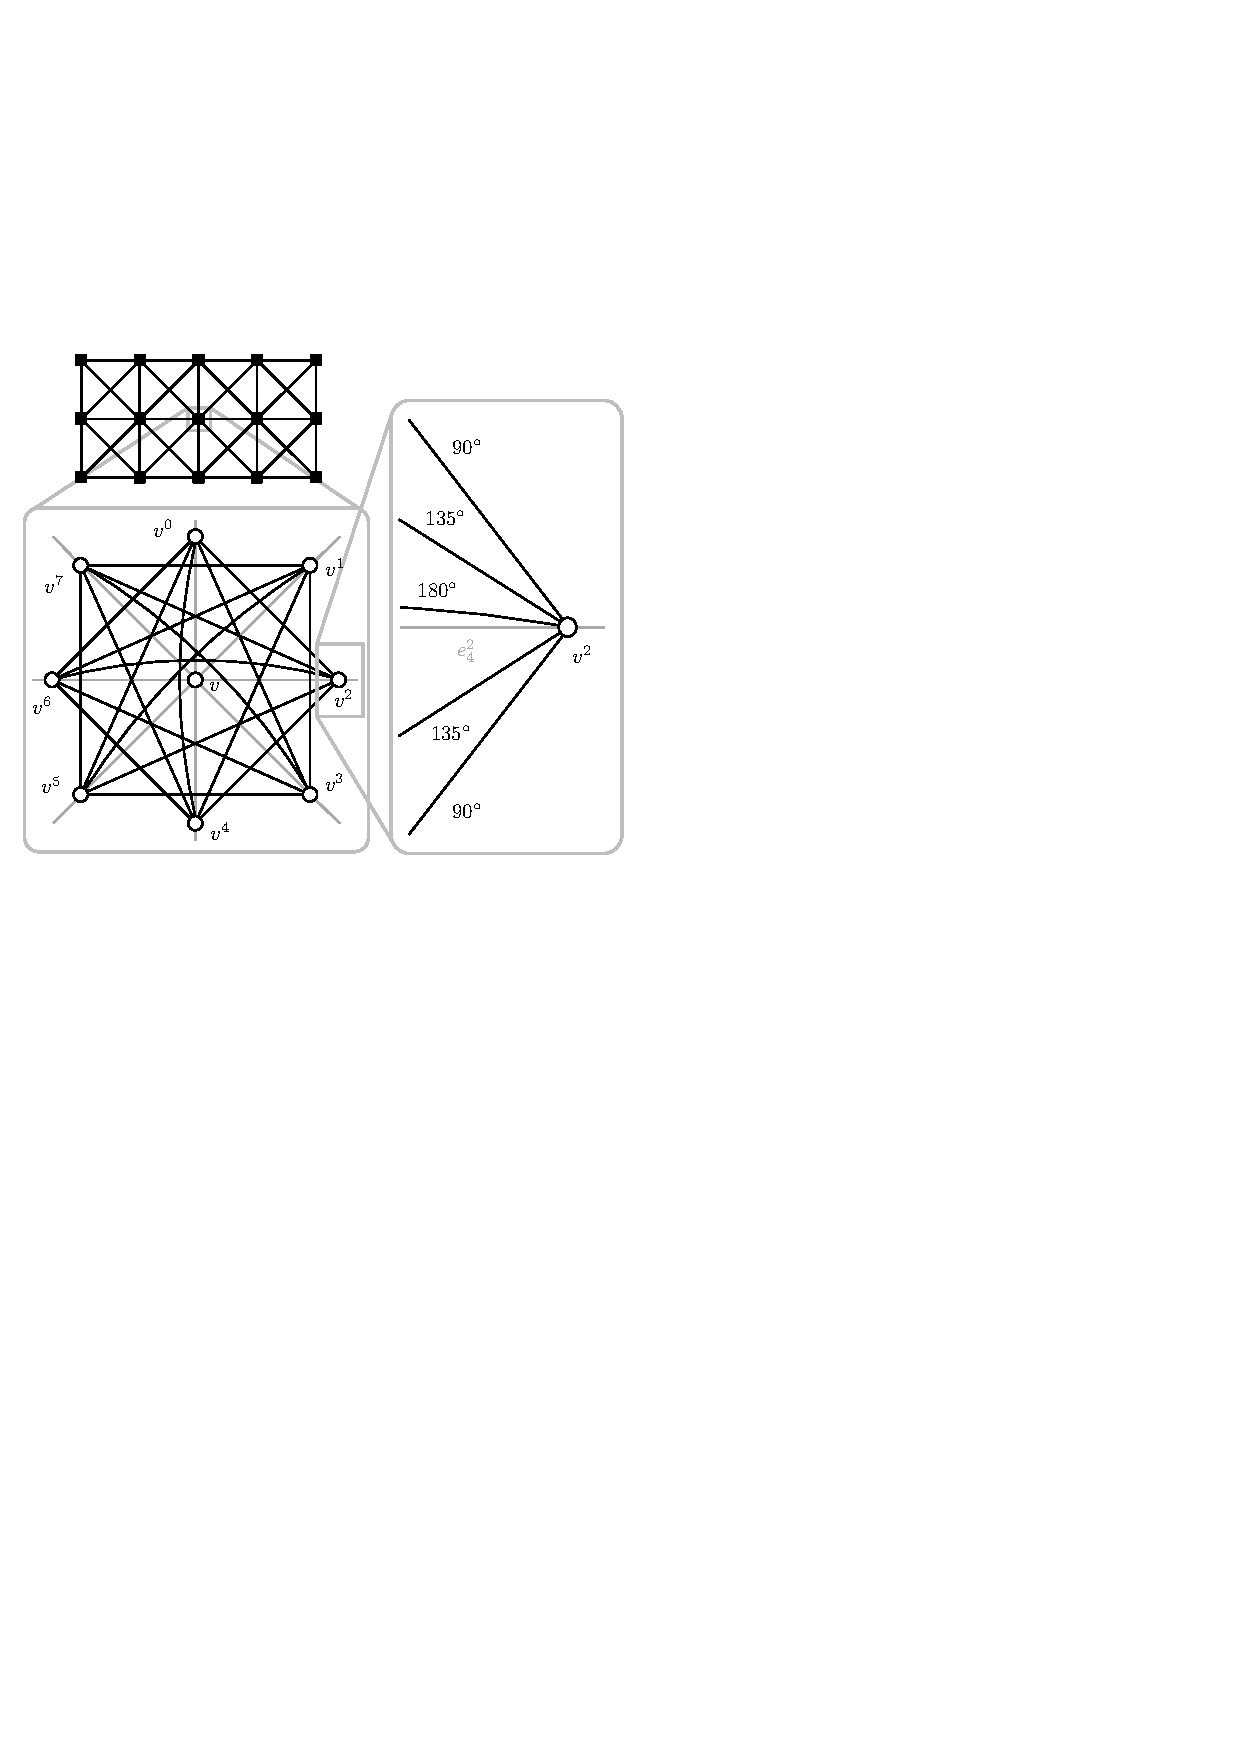
\includegraphics[width=0.45\textwidth]{figures/node.pdf}}}$
	\caption{A $3\times3$ grid graph. Each node $v_i$ has 8 ports $v_i^0 ... v_i^7$ which are connected to $v_i$ by a direct edge. Each port is additionally connected to its $180^{\circ}$, $135^{\circ}$ and $35^{\circ}$ neighbor ports.}
	\label{FIG:gridgraph}
\end{figure}

Following this insight, we introduce a constant $a \geq 0$ and set the port edge costs as follows:
\begin{align}
c_{180} &= a + p_{180} = a \\
c_{135} &= a + p_{135} \\
c_{90} &= a + p_{90} \\
c_{45} &= a + p_{45}.
\end{align}
We choose $a$ in a way such that the following inequalities are fullfilled:
\begin{align}
2a + p_{135} &\geq a + p_{90} \label{CONSTRS:sim90}\\
2a + p_{135} + p_{90} &\geq a + p_{45}\label{CONSTRS:sim45}.
\end{align}
Ineq.~(\ref{CONSTRS:sim90}) ensures that simulating a $90^{\circ}$ pass with two $135^{\circ}$ passes is never cheaper than $c_{90}$. Ineq.~(\ref{CONSTRS:sim45}) ensures that simulating a $45^{\circ}$ pass with a $135^{\circ}$ pass and a $180^{\circ}$ pass is never cheaper than $c_{45}$.

The inequalities are fullfilled for $a = p_{45} - p_{135} \geq 0$, leading to the following port edge costs:

\begin{align}
c_{180} &= p_{45} - p_{135} \\
c_{135} &= p_{45} \\
c_{90} &= p_{45} - p_{135} + p_{90} = c_{180} + p_{90} \\
c_{45} &= 2 p_{45} - p_{135} = c_{180} + c_{135}.
\end{align}

We can thus omit explicit edges for $45^{\circ}$ turns, as they can always be exactly replaced by a $180^{\circ}$ and a $135^{\circ}$ edge.

Figure~\ref{FIG:grids}, left provides two example of paths through an octilinear grid graph.

\begin{figure*}[h]
  \centering
	$\vcenter{\hbox{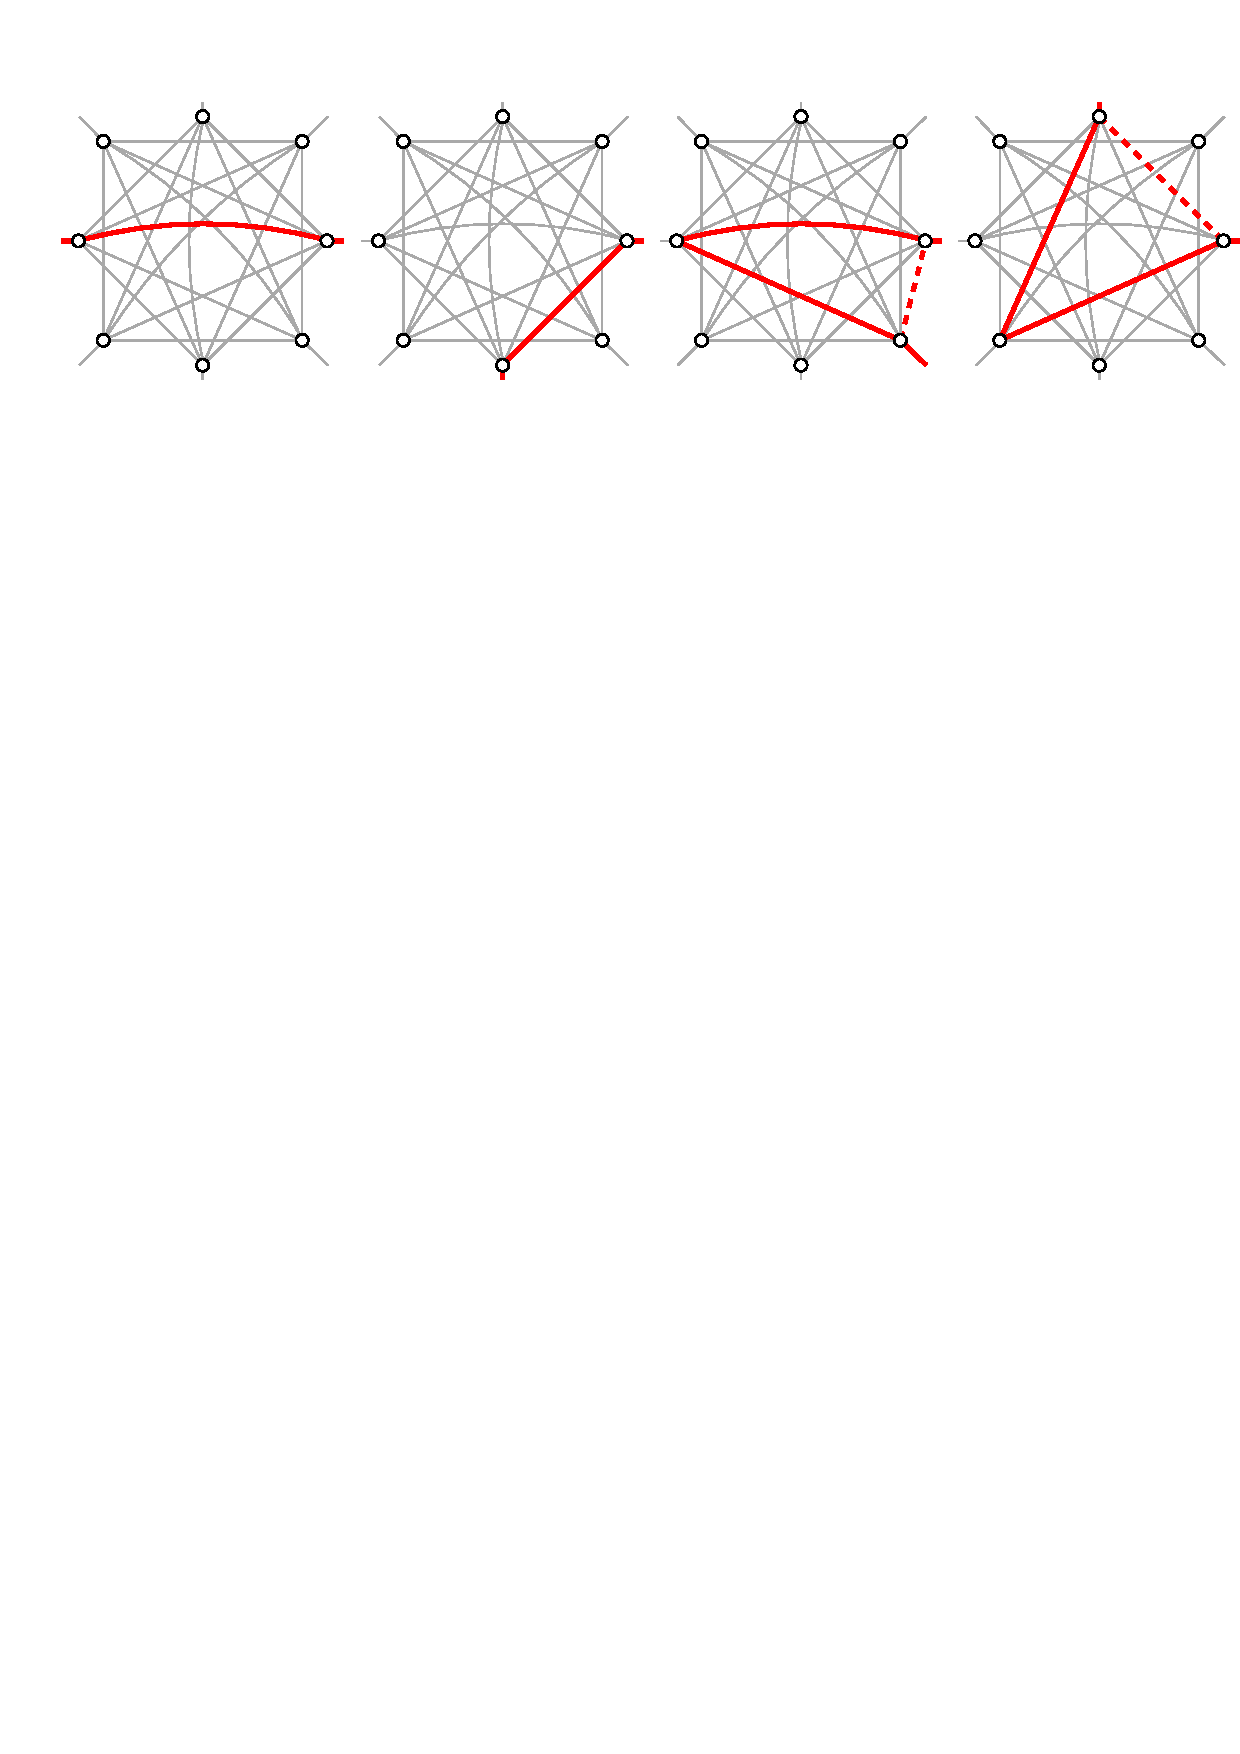
\includegraphics[width=0.9\textwidth]{figures/paths.pdf}}}$
	\caption{1. A $180^{\circ}$ pass through a node $v$. 2. A $90^{\circ}$ pass through $v$. 3. A $45^{\circ}$ pass through $v$ simulated by a $180^{\circ}$ and $135^{\circ}$ pass. 4. A $90^{\circ}$ pass through $v$ simulated by two $135^{\circ}$ passes. }
	\label{FIG:paths}
\end{figure*}

\subsection{Shortest-Path Iteration}

At the core of our approach lies an iterative shortest-path search, using a straight-forward implementation of Dijkstra's algorithm. We recall that the input to our algorithm is an undirected planar graph $G = \{V, E\}$. In a first step, we apply a preprocessing step commonly used in metro map drawing and delete every node from $G$ with degree 2. The adjacent edges are combined into one. In the final octilinear drawing, these removed nodes are then inserted again equidistantly.

We say a an edge $e \in E$ is ``settled'' if $e \in S$ and initialize $S = \emptyset$. Additionally, we define a function $\omega(v) \in V_\omega$ which assigns $v$ the nearest node in $\Omega$.

  The intuitive idea behind our algorithm is to calculate
$|E|$ shortest paths $\left(\omega\left(v\right), \omega\left(u\right)\right)$ in $\Omega$ for each edge $e = \{u, v\}, e \in E$ until all edges are settled. This would already give us an octilinear, locally turn-optimized drawing. The following challenges prevent a straight-forward implementation of this idea:
\begin{enumerate}
\item Edges are not allowed to cross each other in the final drawing.
\item Nodes are not allowed to share positions.
\item The optimal position of a node $v$ in $\Omega$ may not be the grid node which is nearest to $v$, but some other grid node nearby. We have to give $v$ some slack.
\end{enumerate}

We adress the first problem by adding the path found after each iteration as an obstacle to $\Omega$. This is explained in more detail in Sect.~\ref{SEC:balancing}. To adress the second problem, we extend $\omega(v)$ by the following rule: if the grid node nearest to $v$ has already be selected for another node $v' \neq v$, take the nearest unselected grid node from $V_\omega$ that is still within a maximum displacement distance $\hat d_v$.

% TODO: call non-chosen nodes 'free', below and above

To give nodes some slack to snap into an optimal position, we don't actually calculate the shortest path between two nodes $\omega(u)$ and $\omega(v)$ if one of them has not already been chosen in a previous iteration. Instead, but between $\omega(u)$ and all possible target nodes in $\Omega$ that have a distance to $u$ that is less than $\hat d_v$. This can easily be integrated into our shortest-path search - we just abort Dijkstra's algorithm as soon as we have reached \emph{some} of the target nodes. This node is then guaranteed to be the closest of all target nodes to $\omega(v)$ in terms of the cost function. Fig.~TODO gives an example of this approach.

A negative side-effect of this trick is that it tends to move unsettled target nodes to settled source nodes, thus shortening the generated curve and creating a local optimum (Figure X, left). To make our approach stable even for large max. displacement factors, a simple heuristic may be applied. Instead of selecting \emph{every} grid node with a certain maximum distance to $v$ as a possible target node, we additionally restrict these nodes to have a distance smaller than or equal to the distance between the target and the source node (Fig. X, right).

For edges leading to a terminus node ($\deg(v) = 1$), this effect can be utilized to achieve \emph{edge contraction}. A common pattern in transit networks is a dense, convoluted network center, and several suburban lines going out of the center in a star-like fashion. These branches usually have a lower station density than the center lines, and drawing them according to their geography leads to very unbalanced maps. We contract these branches by allowing the branch terminus to be displaced by $0.5$ edge lengths (see Figure 1).

\subsection{Graph Balancing}
\label{SEC:balancing}

After each SP iteration, our grid graph $\Omega$ is balanced \emph{locally}. Locally in this context means that for every edge $e$ present in the shortest path found in the last iteration, we only update edges that can be reached from $e$ in constant time. Additionally, we update the source and the target node of the path (which again can be done in $\mathcal{O}(1)$).

Edge balancing has three objectives:

\begin{enumerate}
\item Transform already settled curves of the final drawing into obstacles in $\Omega$
\item Establish a distance buffer around settled curves
\item Distribute the edge cost of the 8 outgoing edges of the target and source node in a way to optimizes the incident angle of the next settled edge curve
\end{enumerate}

\subsection{Preserving Topology}

\subsection{Input Ordering}

Naturally, the quality of our approach depends heavily on the ordering the edges in $G$ are processed.


\subsection{Complexity}

\section{Evaluation}

\subsection{Penalty Experiments}

\section{Conclusions}

We have described our approach in detail and demonstrated that it produces octilinear metro maps that are not only very close to existing ILP approaches in terms of our quality measure, but also convince esthetically.

However, while problems with local optima may not be as striking as in other non-global techniques, they are still evident. We are confident that the esthetical impact of many of this optima can be significantly reduced by combining our approach with an additional local search optimization strategy at the end of the SP iteration. It may be especially promising to implement our approach itself as an ILP, which would allow for a global optimization of the map, guided by our octilinear grid graph.

\balancecolumns
\end{document}
